%%%%%%%%%%%%%%%%%%%%%%%%%%%%%%%%%%
% 01_Introduction                %
%%%%%%%%%%%%%%%%%%%%%%%%%%%%%%%%%%

\chapter{Introduction}

SBMLsimulator \citep{Doerr2014a} is a easily usable, portable, and powerful simulation, visualization, and parameter optimization engine for biochemical network models in \SBML format \citep{M.Hucka03012003}.

\SBML is a file format that stores systems biology models in a structured way.
The main idea behind \SBML is that a model should always yield identical results, no matter which software was used to build the model.
SBMLsimulator got its name from this file format.

SBMLsimulator uses the \SBSCL \citep{Keller2013}, which is based on \JSBML \citep{Draeger2011, Rodriguez2015}, as its computational core and combines its functions with \EvA \citep{Kron10EvA2}, a \Java framework for nature-inspired heuristic optimization procedures.
In this context, optimization means the estimation of model parameters, \ie the calibration of a model with respect to given experimental data \citep{Draeger2009a}.

As the name suggests, SBMLsimulator was initially developed to provide an intuitive graphical user interface for loading \SBML models, running simulations, and plotting the results.
With version 2.0, its capabilities greatly expanded: SBMLsimulator comes with a comprehensive visualization implementation. 
This feature makes it possible to dynamically visualize experimental and simulated data in the context of biological networks in form of \SBGN process diagrams \citep{Rougny2019}.

Just like \SBML that has been developed for encoding models of biological systems in a structured way, \SBGN brought important design principles to the models.
The aim of \SBGN is that biological networks can be drawn in a standardized fashion, thereby removing any potential ambiguity.

This document is intended to guide you through the function and use of SBMLsimulator.
We will start by explaining how to install and launch the program, and how to use its more advanced features.

Now, we briefly discuss the main features of SBMLsimulator, before the next chapter gets us started by installing the program on your computer.

\section{Main program features}

SBMLsimulator has been designed to
\begin{dinglist}{52}
\item parse \SBML files and display its content in a \GUI for exploration.
\item insert missing values into the model that are required to perform a dynamic simulation.
\item interpret metabolic, gene regulatory, and signal
transduction models in terms of an \ODE systems and solve those with numerical integration methods.
\item fit the model to given experimental data and save the optimization results in the model.
\item plot experimental and simulation data, \ie temporal changes of all model components.
\item export simulation results as \CSV or image file.
\item save user preferences and restore all your settings when launched next time.
\item be launched as a \Garuda gadget from the \Garuda dashboard \citep{Ghosh2011}.
%\item be used as a \JavaWebStart application without any local installation of software, directly from the website in your browser or by clicking at this link: \href{http://www.cogsys.cs.uni-tuebingen.de/software/SBMLsimulator/downloads/SBMLsimulator-latest.jnlp}{SBMLsimulator-latest.jnlp}.
\item be used in a command-line mode without \GUI.
%This is, for instance, useful for large-scale parameter estimation.
\item be embedded as an \API in a third-party program, allowing to access all of its functions in more complex scripts and procedures.
\item draw network layouts based on the information provided in loaded \SBML files or to automatically generate \SBGN process diagrams in cases where the \SBML files do not contain any layout information.
\item to map data that may originate from biological experiments or from computer simulation onto \SBGN network diagrams
\item to allow users zooming and panning while dynamic animations are proceeding.
\item to generate snapshot images or animated videos from the data mapping, including an implementation of a Ken-Burns effect (sliding view port window).
\end{dinglist}


%%%%%%%%%%%%%%%%%%%%%%%%%%%%%%%%%%
% 02_Installation                %
%%%%%%%%%%%%%%%%%%%%%%%%%%%%%%%%%%

\chapter{Installation}

To obtain a copy of SBMLsimulator, we open a web browser and navigate to the Github page of the Dräger research group at \github{draeger-lab/} and go to \href{https://github.com/draeger-lab/SBMLsimulator/}{SBMLsimulator}. When we click on ``\href{https://github.com/draeger-lab/SBMLsimulator/releases/}{releases},'' we can find the latest release on top, currently SBMLsimulator 2.0.
\watchAtYoutube{Eu4uSPmNXVI}

SBMLsimulator comes in two different versions: As a stand-alone \JAR file or as a gadget for users of the \Garuda platform that is available from \href{http://garuda-alliance.org}{\texttt{garuda-alliance.org}}.
Once we embed the correct version of SBMLsimulator in our \Garuda installation folder, we can launch the application from the \Garuda dashboard or from any other \Garuda-enabled software.

Let us download the \JAR file and launch the application with a double click within our downloads folder.
To run SBMLsimulator, we need to have the \JVM installed on our computer, which Oracle provides for personal or commercial use\footnote{\url{https://www.java.com}}, or its open-source pendant\footnote{\url{https://openjdk.java.net}\label{fn:jvmldl}} for all other purposes.

\section{Requirements}
\subsection{Software}

SBMLsimulator is entirely written in \Java and runs on any desktop \OS
where a suitable \JVM is installed (\JDK version 8 or newer), including \Windows, \Linux, and \MacOSX.
Version 2.0 of SBMLsimulator has been tested on \Windows~10, OpenSuSE Tumbleweed (version December 20191228), and
%\Windows~7 to \Windows~10, \Linux (Ubuntu 10.04 LTS and OpenSuSE Tumbleweed version \TODO{XXX}), and 
\MacOSX versions 10.14.6 (Mojave) and 10.15.2 (Catalina).
See, for example, the \Java SE download
page\footref{fn:jvmldl}.
If you encounter any issues with your \OS, the \cref{ch:faq} might provide answers to you.
To report problems or bugs, it is recommended to use the project's issue tracker at \github{draeger-lab/SBMLsimulator/issues/}.


\subsection{Hardware}

With at least \SI{1}{\giga\byte} main memory, we should be able to perform most tasks
without any problem.
SBMLsimulator runs without an active internet connection.

\section{Starting the application}
\label{startingTheProgram}

\begin{wrapfigure}{O}{.81cm}
\vspace{\wrapfigspace}

\includegraphics[width=.8cm]{jar_icon}
\end{wrapfigure}
If we downloaded a ZIP-file, we need to unzip it before starting the application.
In the most simple case, we can launch SBMLsimulator by double-clicking at the \Java application icon (see image next to this text).
SBMLsimulator can run out-of-the-box on all systems where a \JVM is installed and does not require any further installations.
When launching the application, opens with a splash screen indicating the version number.

We can also start the application on all desktop \OS by typing the following on the command prompt:
\begin{lstlisting}[language=bash,numbers=none]
  java -jar -Xms128m -Xmx1024m SBMLsimulator_v<version.number>.jar
\end{lstlisting}
Please note that we might have to change
\texttt{<version.number>} to the actual name of the \JAR we downloaded, \eg \texttt{SBMLsimulator\_v2.0.jar}.
In this example, we pass arguments to the \JVM to make a minimum of \SI{128}{\mega\byte} and a maximum of \SI{1024}{\mega\byte} of memory available to the program.
In most cases, SBMLsimulator needs more than \SI{128}{\mega\byte} of memory, so it might be convenient to create a shortcut and start the application with as much memory as available.
If we have \SI{2}{\giga\byte} of \RAM, for example, we might want to start the application with the command shown in \cref{lst:launch}.
\begin{lstlisting}[language=bash,numbers=none,captionpos=t,float=b,caption={Launching SBMLsimulator from the command-line with additional memory},label={lst:launch}]
  java -Xms128m -Xmx1400M -jar SBMLsimulator_v<version.number>.jar
\end{lstlisting}
This small example already indicates that launching the program from the command-line has some advantages compared to double-clicking the icon, namely that we can pass so-called ``command-line arguments'' not only to the \JVM, but also directly to the program.
These allow us, for instance, to directly open a specific model file when launching the application or customize many other settings.
SBMLsimulator shows us an overview of all available command-line options when adding \texttt{-?} to the start command (see \cref{chap:CMD} for details).

To simplify matters, we could create a start-scripts to run the application with as much memory as possible.
How much memory is actually needed strongly depends on the size of our input datasets.

SBMLsimulator is a bi-lingual program, which has been translated to \German in addition to its \English user interface.
When launching the program, it uses English, unless our \OS has a \German environment.
We can select the language of the program by passing the parameter \texttt{-Duser.language=en} to the \JVM upon the start of the program if we like to have an \English user interface, or \texttt{de} for the \German interface.

Now that we got SBMLsimulator installed and running on our computer, we will explore its use in the following chapters.

%%%%%%%%%%%%%%%%%%%%%%%%%%%%%%%%%%
% 03_Getting_Started             %
%%%%%%%%%%%%%%%%%%%%%%%%%%%%%%%%%%

\chapter{Loading model files and running a simulation}%{How to get started}

In this chapter, we will discuss selected features of the software SBMLsimulator.
First, we will start by explaining where to find systems biology models, how to load them into the application, and how to run a simulation.
\watchAtYoutube{CVzp\_XtIaHU}
We will then discuss a more advanced feature, namely the calibration of model parameters with respect to experimental data.

\section{Obtaining an example model}

Several online repositories exist that house systems biology models.
Let us explore how we can get the dynamic model of human hepatocytes that \citeauthor{Bucher2011} published in \citeyear{Bucher2011} in \emph{BMC Systems Biology} from an online database in \SBML format.
We open a web browser and enter \href{http://www.ebi.ac.uk/biomodels/}{\texttt{biomodels.net}} in the address bar, which redirects us to \BioModels \citep{Malik-Sheriff2019} hosted at the European Bioinformatics Institute, or EBI.

Since we are interested in a specific model, we can simply enter some keywords in the search field, such as ``Bucher hepatocytes'' and click at the magnifying glass.
And here is the result with model identifier \numero \href{https://identifiers.org/biomodels.db/BIOMD0000000328}{328}.
The tab ``Files'' provides several downloads to us, of which the model file in \SBML format is most interesting to us for now, which is listed at the top.
Note that \SBML files can have various file extensions.
Most common are \texttt{.sbml} or, as it is here, \texttt{.xml}.
One click and we should have the model in our \directory{Downloads} folder.

Many other published models available from the \BioModels website\footnote{\url{http://www.ebi.ac.uk/biomodels-main/publmodels}} have been curated by a team of experts.
If we like to download a model, click the respective \ac{Id}, which brings us to a page containing a description of the model and a button ``Download SBML.'' 
We position the cursor at this button and then we see the possible \SBML levels and versions to download.
If we click on the respective combination of level and version, the desired \SBML file will be downloaded.

Alternatively, we can also create an \SBML model ourself.
To this end, dedicated software solutions, such as \CellDesigner \citep{Funahashi2008} can be used.
For downloading CellDesigner please go to the project's website\footnote{\url{http://www.celldesigner.org}}.

\section{Loading, exploring, and simulating a kinetic model}

In order to perform model simulations, we first need to load an \SBML model. 
If we additionally want to compare the simulation results to experimental data or run a parameter estimation, it is required to also load the experimental data into SBMLsimulator.
In our example, we generate artificial data from the example model.
We can obtain artificial data, too, by running a simulation with SBMLsimulator and exporting the numerical solution to a \CSV file.
This procedure is explained in detail below.

\subsection{Open a model file}
\begin{wrapfigure}{O}{16px}
\vspace{\wrapfigspace}

\includegraphics[width=16px]{folder_64}
\end{wrapfigure}
We can simply drag \& drop the model file (an \SBML document) into the application or select \menu{File > Open > Open model}  to load a model (see \cref{fig:openModel}).
Another option would be to click at the folder icon in the tool-bar, which is displayed next to this text.
Depending on our \OS, we can also use the key stroke combinations \keys{\cmd + O} (\MacOSX) or \keys{\ctrlwin + O} (\Linux and \Windows).
SBMLsimulator memorizes up to ten previously opened \SBML documents in the menu under \menu{File > Recent files}, where the most recently used file will appear at the top most position.
To open one of the ten previously loaded models, we can also use the keystroke combinations \keys{\Altmac} or \keys{\Altwin + 0} to \keys{9} (\OS-dependent).

\begin{figure}[t]
\centering
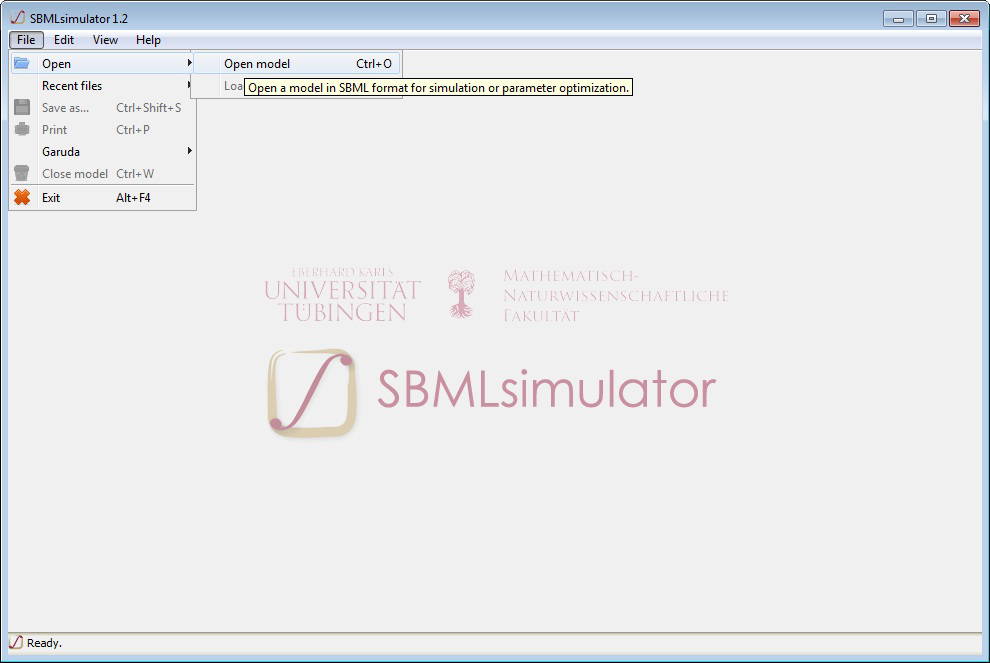
\includegraphics[width=\textwidth, trim={0 .75cm 0 0}]{open_model}
\caption[Loading of a model]{Loading of a model.
One possibility to open a model is to select \menu{File > Open > Open model}.
Depending on our \OS we can also use one of the following keystroke combinations \keys{\cmd + O} (\MacOSX) or \keys{\ctrlwin + O} (\Linux and \Windows).
To open one of the ten recently opened models, we can select \menu{File > Recent files}.}
\label{fig:openModel}
\end{figure}
\begin{figure}[t]
\centering
\shadowimage[width=\textwidth]{opened_model}
\caption[SBMLsimulator with a loaded model]{SBMLsimulator with a loaded model.
In this window we can choose the simulation settings (bottom), the parameter values (center left), and the quantities to plot (upper left).
The plot section is on the right.}
\label{fig:modelOpened}
\end{figure}

\subsection{Graphically exploring a model}
\label{sec:ModelTree}

Now, the model is loaded and the window's appearance changes as \cref{fig:modelOpened} shows:
\begin{dinglist}{226}
  \item The right part of the window is for plotting simulation results and experimental data points (if experimental data has been loaded).
In the bottom part of the window we can determine simulation preferences like the solver or the number of simulation steps and the quality function for comparing experimental data (if present) to simulation results.
  \item In the center left part of the window the compartment values, the initial values of the reactive species, and parameter values in the model can be changed.
  Please note that after typing a new value in, the change only takes effect after we either press the return key \keys{\return} or the tabulator key \keys{\tab}.
  \item The upper left part is for choosing the quantities that should appear in the plot.
\end{dinglist}
The user interface of SBMLsimulator comprises several tabs.
In the \menu{Model} tab, we can explore the structure of the model in a tree view, including all of its components, such as compartments, species, parameters, or reactions.
\Cref{sec:ModelTree} discusses the content of this tab in detail.
The \menu{Graph} tab visually displays the model, which may look like \cref{fig:AutomatedLayout}.
In case of the example model by \citeauthor{Bucher2011}, the authors did not embed any layout information into their model and SBMLsimulator has hence to automatically generate a display following the \SBGN guidelines.
\Cref{chap:VisLayout} discusses this feature in more detail.
\begin{figure}[htb]
  \shadowimage[width=\textwidth]{Automatic_Layout}
  \caption[Example for an automatically generated layout of a metabolic network model]{Example for an automatically generated layout of a metabolic network model.
  When loading an \SBML file without embedded layout information, SBMLsimulator tries to automatically generate a graph display in the style of an \SBGN process diagram.
  This example shows one such layout generated from the model by \citeauthor{Bucher2011}.}
  \label{fig:AutomatedLayout}
\end{figure}

\begin{wrapfigure}{o}{16px}
%\vspace{-4ex}%\wrapfigspace}
%\begin{minipage}[t][20px][c]{25px}
%\parbox[r][20px][c]{20px}{

\includegraphics[width=16px]{search_64}%}
%\end{minipage}
\end{wrapfigure}
We can explore the tree structure of the model if we choose the tab \menu{Model}, where we see the \SBML document in a tree structure that we can explore (\cref{fig:modelTree}).
A search function at the bottom gives us the opportunity to browse the model for any of its components.
Here we can search for \acp{Id} or names of components, for instance, all Michaelis constants ($K_M$ values) in the model.
The tree will be expanded and elements that do not match our filter criteria will be removed from the view.
When clicking at individual model components, the program displays detailed information about the selected element.
\begin{figure}[t]
\centering
\shadowimage[width=\textwidth]{model_tree}
\caption[Display of model tree]{Display of model tree.
The model tree is shown when clicking on the \menu{Model} tab.
We can explore the model by clicking at elements within the tree.}
\label{fig:modelTree}
\end{figure}


\section{Dynamic simulation of a model}
\begin{wrapfigure}{o}{16px}
\vspace{\wrapfigspace}

\includegraphics[width=16px]{PLAY_64}
\end{wrapfigure}
Next, let us run a dynamic simulation, \ie interpret the model in terms of an \ODE system.
At the bottom is a control panel where we can adjust how the simulation should be performed, for instance, with 300 steps.
We can also select the solver that calculates the result for us.
SBMLsimulator offers a large variety of integration routines for this purpose.
The default solver, ``Rosenbrock,'' is the most precise method and solves the broadest range of models.
However, its high preciseness comes at the cost of a generally higher run time compared to the other solvers.
\Cref{tab:solvers} lists all solvers that SBMLsimulator provides together with a short description and a reference for more information.
When clicking the run button at the top, as \cref{fig:startSimulation} shows, the calculation starts.
\begin{figure}[t]
\centering
\shadowimage[width=\textwidth]{select_species}
\caption[Selection of quantities for plotting]{Selection of quantities for plotting.
We can, for instance, click on \menu{Select > Species} in order to choose all species for plotting.}
\label{fig:selectSpecies}
\end{figure}
\begin{figure}[t]
\centering
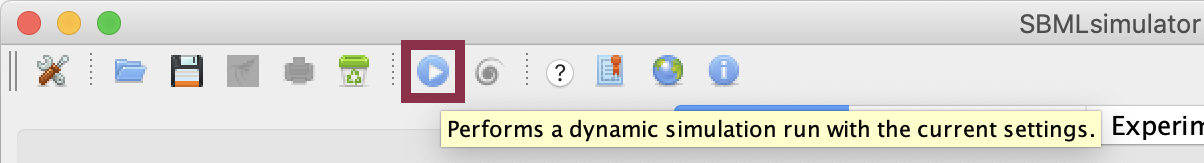
\includegraphics[width=\textwidth]{start_simulation}
\caption[Starting of a simulation in SBMLsimulator]{Starting of a simulation in SBMLsimulator.
By clicking on the simulation button, the simulation of the model is started.}
\label{fig:startSimulation}
\end{figure}
\begin{figure}[t]
\centering
\shadowimage[width=\textwidth]{simulation_results}
\caption[Simulation results plotted in the right panel of the window]{Simulation results plotted in the right panel of the window}
\label{fig:simulationResults}
\end{figure}

Once the computation has finished, we can see all selected model components in the plot area.
On the left panel in the \menu{Simulation} tab, we can select, for which model components the simulation results should be added to the plot diagram.
To this end, we click at the individual check boxes for model components of interest.
The buttons \keys{Select} and \keys{Deselect} give us the choice to visualize or remove an entire group of elements from the plot, such as all species or all fluxes.
In \cref{fig:selectSpecies}, for instance, we select to plot all species values.
\Cref{fig:simulationResults} shows us the result for this model simulation.
Selecting model components is necessary, because SBMLsimulator does not know which model components we like to display in the plot area.

When finishing a simulation run, the tab \menu{Computed data} becomes active, where we can see the simulated time course from the plot in tabular format.

With the availability of this data set, the graph view in the \menu{Graph} has now also updated and automatically maps the simulated data onto the generated network.
We can play these data as a movie, zoom in, and pan the system around while it is running.
The controls at the bottom adjust the properties of this animation.
\Cref{chap:VisLayout} gives more details of this feature.

The view in \menu{Simulation} also gives us the opportunity to play with the initial values or parameters in the model in the panel to the left.
For instance, we might be interested in setting a new value for some Michaelis parameter ($K_M$ value), and see how the results of the simulation change after rerunning the model.
If we have a time-course data set from laboratory experiments available, we can load it into SBMLsimulator and apply a plethora of heuristic optimization methods to automatically estimate optimal values of such model parameters.
\Cref{chap:ParameterEstimation} explains this is a topic in detail.

\begin{wrapfigure}{o}{16px}
\vspace{\wrapfigspace}

\includegraphics[width=16px]{STOP_64}
\end{wrapfigure}
If in some cases a simulation run consumes too much time, we can always interrupt it by clicking at the stop button in the tool-bar (see image at the side of this text), which is activated whenever we launch a simulation.

\rowcolors{2}{white}{lightsilver}
\begin{longtable}{C{3.3cm}p{11cm}}
\hiderowcolors
\caption[Available ODE solver implementations]{Available ODE solver implementations}
\label{tab:solvers}\\
\toprule
Solver & Description\\
\midrule
\endfirsthead
\caption{Available ODE solver implementations (continued)}\\
\toprule
Solver & Description\\
\midrule
\endhead
\multicolumn{2}{c}{\small Continued on the next page\dots}
\endfoot
\bottomrule
\endlastfoot
\showrowcolors
Adams-Bashforth
\citet{ApacheCommonsMath2013}&
This is an explicit multi-step integration method.
The solver uses a step-size adaptation.
It is faster than Rosenbrock, but not applicable for very stiff differential equation systems.
This solver is provided by Apache Commons.\\
Adams-Moulton
\citep{ApacheCommonsMath2013}&
The method by Adams and Moulton is an implicit multi-step integration method, which uses a step-size adaptation.
It is also faster than Rosenbrock, but not applicable for all models.
This solver is provided by Apache Commons.\\
Dormand-Prince 54
\citep{ApacheCommonsMath2013}&
The Dormand Prince in an explicit integration method of order 5, which belongs to the family of Runge-Kutta methods.
Step-size adaptation is included in the routine.
This solver works for most models, but can have problems with extremely stiff differential equation systems.
It is provided by Apache Commons.\\
Dormand-Prince 853
\citep{ApacheCommonsMath2013}&
This solver is similar to Dormand-Prince 54, but it is of order 8.
It comprises more function evaluations than Dormand-Prince 54 and is therefore more precise, but also slower.
It is provided by Apache Commons.\\
Euler
\citep{Press1992}&
The explicit Euler method.
This is a very fast and simple solver, that lacks a step-size adaptation and might, therefore, be imprecise.\\
Gragg-Bulirsch-Stoer\newline
\citep{ApacheCommonsMath2013}&
This method belongs to the most efficient and accurate methods with step-size adaptation for non-stiff differential equations.
Its use is not recommended for stiff differential equations.
This solver is provided by Apache Commons.\\
Higham-Hall 54
\citep{ApacheCommonsMath2013}&
The method by Higham and Hall is a Runge-Kutta method of order 5 with step-size control.
The solver is similar to the Dormand-Prince 54 solver.
It is provided by Apache Commons.\\
Rosenbrock\newline
\citep{Press1992}&
This adapted solver comprises Rosenbrock's method, which includes an adaptation of step-size.
This implementation is specifically dedicated to precise simulation of \SBML models and is applicable for very stiff differential equation systems. But it might be significantly slower for some models than the other solvers.\\
Runge-Kutta\newline
\citep{Press1992}&
The classical fourth order Runge-Kutta method.
It is fast, but imprecise for many models, as it does not contain a step-size adaptation.
\end{longtable}


\subsection{Save simulation data}
\label{ch:savesim}
\begin{wrapfigure}{O}{16px}
\vspace{\wrapfigspace}

\includegraphics[width=16px]{save_64}
\end{wrapfigure}
Saving information from the \GUI is context-sensitive in SBMLsimulator: Depending on which tab is selected, we can save different pieces of information.
If we want to save computed data from a simulation, we need to select the tab \menu{Computed data} first (see \cref{fig:saveSimulationResults}).
Then we can save the simulation data under \menu{File > Save as}.
Just like for the plot data, we can also use keystroke combinations to save our simulation data. To this end, just select the tab \menu{Computed data} and hit the keys \keys{\cmd + \shift + S} if we are working under \MacOSX, or \keys{\ctrlwin + \shift + S} for \Linux and \Windows.
\begin{figure}[b]
\centering
\shadowimage[width=\textwidth]{save_simulation_results}
\caption[Table with simulation data]{Table with simulation data.
Under the tab \menu{Computed data} we can see the simulation results in a table.
They can be saved under \menu{File > Save as}, by clicking the floppy icon in the tool-bar, or by using an \OS-dependent keystroke combination.}
\label{fig:saveSimulationResults}
\end{figure}

%\newpage
\subsection{Save plot image}
\begin{wrapfigure}{o}{16px}
\vspace{\wrapfigspace}

\includegraphics[width=16px]{PRINT_64}
\end{wrapfigure}
If we like to save the current plot as an image, just select the tab \menu{Simulation}.
We can then save the image of the results plot by clicking at \menu{File > Save as}.
For users who prefer keystroke combinations, it is also possible to save the plot by hitting the keys \keys{\cmd + \shift + S} if we are working under \MacOSX, or \keys{\ctrlwin + \shift + S} for \Linux and \Windows.
By clicking at the printer icon (displayed next to this text) we can print the current plot or save it as a \PDF.
The print function can also be used with the keystroke combination \keys{\cmd + P} (\MacOSX) or \keys{\ctrlwin + P} (\Windows and \Linux).


\section{Next steps}

We have now walked through how to load a model and run a simulation using SBMLsimulator.
In \Cref{chap:ParameterEstimation}, we will explore how to automatically estimate parameter values.
In other words, this will explain how a model can be calibrated with respect to experimentally obtained time-course data.
After discussing how to embed manually created network layouts in \SBML files in \Cref{chap:EmbeddingLayoutsInModels}, \cref{chap:VisLayout} will then focus on how to create dynamic videos of metabolic networks that you can use for visual analytics or embed within scientific presentations.


%%%%%%%%%%%%%%%%%%%%%%%%%%%%%%%%%%
% 04_Parameter_Estimation        %
%%%%%%%%%%%%%%%%%%%%%%%%%%%%%%%%%%

\chapter{Parameter estimation}
\label{chap:ParameterEstimation}

In many cases, biological models contain quantities with uncertain values.
These values must be estimated by calibrating the model with respect to given experimental data.
To facilitate this complicated procedure, SBMLsimulator comes with the optimization toolbox \EvA that provides a large collection of nature inspired heuristic optimization procedures, \eg \ES \citep{Rechenberg1973, Schwefel1975}, \GA \citep{Holland1975}, \DE \citep{Storn96Usage}, or \PSO \citep{ClercKennedy02, Clerc2005} and \Tribes \citep{Clerc2006}, as well as niche-based methods that have been found to be particularly useful for applications in systems biology \citep{Kron09NichingGCB}.


\section{Preparing and loading measured data}
\label{ch:prepare}

First of all, we will need to load a time-course data set into SBMLsimulator that we can use for calibrating our model of interest.
The idea is that for every measured quantity from the data set the distance of the simulation results to the measured values should be minimized.
To load the data into SBMLsimulator, we need to make sure that our experimentally measured data set conforms the required file format.
The application reads \CSV files, which are mostly tab- or comma-separated files of data.

\subsection{Exporting \CSV files from spreadsheet software}
\label{sec:CSVformat}

Modern spreadsheet software, such as \Excel, \GoogleTables, \LibreCalc, \AppleNumbers, etc., supports exporting data to \CSV.
We are here exemplarily walking through the process for the most widely used software, \Excel.
In other tools, the procedure follows similar steps.

To use data from \Excel, we can simply open our \Excel spreadsheet, click \menu{File > Save as} and select ``Tab-separated text file.''
For all files, the application requires one column called \texttt{time} to be present.
This column should contain for each row the time point it refers to.
Note that the headline of the file must be indicated with a leading pound symbol (\texttt{\#}).
The other columns should be called with the \ac{Id} of the respective quantity in the model and should contain the measured values at the time points, or \NaN if the measurement for a time point is missing. 

Hence, we need a column with the time points and multiple columns that state the values
%(often concentrations)
of each quantity at each time point.
The corresponding \SBML file defines the units of these quantities, so that we do not have to make units explicit in our \CSV file.
The \cref{lst:input:exp} displays an example how an input file may look like.
\begin{lstlisting}[caption={Input file example for experimental data},label={lst:input:exp},numbers=left,captionpos=t,float=t]
#time   s1          s2          s3
0       32.456E-12  7.02        12E32
4       5E-54       179.05E-14  0.005
...     ...         ...         ...
\end{lstlisting}

\subsection{Importing the measured data from a file}
\label{sec:opendata}

In general, all data must be processed time-course data in tabular text files (see \cref{sec:CSVformat} for descriptions and examples of the input file formats).
Just like in the case of model files, we now have several different ways how to open one or more of these datasets in SBMLsimulator: We can
\begin{itemize}
  \item drag \& drop the data file(s) into the application.
  \item select \menu{File > Open > Load experimental data} to open one or multiple files.
  \item use the key stroke combination \keys{\cmd + O} or \keys{\ctrlwin + O} depending on our \OS.
\end{itemize}
Please note that we cannot open experimental data before loading a model.
This is because an \SBML file can contain various meta-data about model components (such as units), whereas the simple \CSV format might not suffice to build the complex data structure for the display.
If we open multiple data files, median values will be used for parameter estimation in each time point.

\Cref{fig:inputdialog} shows an example of the file input dialog.
Here, we open the simulation data saved in \cref{ch:savesim}.
The displayed data set has been restricted to the quantities that \citeauthor{Bucher2011} experimentally measured for their parameter estimation.
SBMLsimulator tries to automatically determine which column from our data file belongs to which model component based on the \acp{Id}.
Only in case of \ac{Id} mismatches, we may need to specify the content of each column in the table at the bottom of the import dialog.
In these cases, we have to click on the combo box below the captions.
\begin{SCfigure}%\begin{figure}[h]
%\centering
\shadowimage[width=.625\textwidth]{import_dialog}
\caption[Example for the data import dialog]{Example for the data import dialog.
The ``CSV Options'' panel can be expanded to correct auto-detected input file properties.
Where needed, the table at the bottom of the import dialog allows us to specify the matching of each column from the data file to a corresponding model component.}
\label{fig:inputdialog}
\end{SCfigure}

SBMLsimulator also tries to automatically infer the format of the data file, \eg what character is used to separate the columns, the character encoding of the file, etc.
If the input file format cannot be automatically inferred (which is not the case in our example here), we may click on the black ``CSV Options'' label to specify further options (like ``column separator char'' or, if the file contains headers, see \cref{fig:csvoptions}).
\begin{SCfigure}%\begin{figure}[h]
%\centering
\shadowimage[width=.625\textwidth]{expanded_csv_options}
\caption[Expanded ``CSV Options" allow to give details for the input file]{Expanded ``CSV Options'' allow to give details for the input file.
These properties are auto-detected and only need to be changed if the auto-detection failed to correctly infer those properties.}
\label{fig:csvoptions}
\end{SCfigure}
After the experimental data are imported, the plot shows the data points as dots (see \cref{fig:simulationResultsWithData}) or in form of box plots in the case we opened more than one data file (not shown).
\begin{figure}[t]
\centering
\shadowimage[width=\textwidth]{simulation_results_with_data}
\caption[SBMLsimulator after simulation and loading of measured data]{SBMLsimulator after simulation and loading of measured data.
The plot shows the simulation results and the experimentally measured data points as dots.}
\label{fig:simulationResultsWithData}
\end{figure}

\section{Defining a quality function}
\label{sec:QualityDefinition}

Before we can calibrate our model to our time-course data set(s), we need to briefly discuss what we consider an optimal solution.
The main idea is that when simulating a calibrated model, we should obtain curves that are as close as possible to experimentally observed values.
In other words, the distance between the calculate behavior of every model component and corresponding data should be minimal.
For instance, if we have measurement data available for the overall intracellular citric acid concentration, the model should yield very similar curves for this reactive species as well.

Model calibration now means that we have to choose values for parameters or initial values for unknown model components such that this difference becomes minimal.
Minimal here means that we have to minimize a distance function.
SBMLsimulator brings with it a selection of distance functions to choose from, which are in analogy to biological evolution also called \emph{\fitness} functions:
\begin{enumerate*}[label=(\roman*)]
  \item (Relative) Euclidean distance,
  \item (Relative) Manhattan distance,
  \item (Relative) N-Metric,
  \item Pearson Correlation, and
  \item \RSE.
\end{enumerate*}
For first attempts or without prior knowledge about the structure of the solution space, it is recommendable to use either the \RSE.
The \RSE has the advantage that higher concentrated substances in the cell do not dominate the quality of the solution because this formula weights the contributions of all model components based on their abundance.
Care must be taken if some model component is known to take a value of exactly zero at any time, because in this case, the \RSE would not be defined.
To circumvent this problem, SBMLsimulator provides a sufficiently high default value, which we can adjust to our needs within the \menu{Preferences} menu.

The panel at the bottom in the \menu{Simulation} tab contains a drop-down menu where we can select an appropriate \fitness function.
The \RSE is selected by default.


\section{Launching the heuristic optimization workbench \EvA}
\label{sec:LaunchingEvA}

\begin{wrapfigure}{o}{16px}
\vspace{\wrapfigspace}

\includegraphics[width=16px]{EvA2_icon}
\end{wrapfigure}
Now that we have loaded a model and corresponding time-course data into SBMLsimulator, the estimation button becomes active in the tool-bar (see the icon next to this text), and does also the corresponding entry in the menu: \menu{Edit > Optimization}.

After clicking either a window like the one shown in see \cref{fig:quantitySelection} appears, in which we can select which quantities from the model to estimate.
Since computational models may contain large numbers of potential optimization targets, the dialog presents them in the four tabs \menu{Compartments}, \menu{Species}, \menu{Global Parameters}, and \menu{Local Parameters}.
Each of these tabs has two buttons at the bottom that allow us to select all quantities within this tab or to deselect them all at once.
If we like to just select a few variables as estimation targets, a search function at the bottom allows us to narrow down the content of the table.
For every estimation target, we can also define their allowable ranges.
Note that we here distinguish between a range for initialization and boundaries for the complete search space.
This distinction can help to generate stable initial solutions and to find allowable values more efficiently.
\begin{figure}[t]
\centering
\shadowimage[width=\textwidth]{select_quantities}
\caption[Selection of quantities to estimate]{Selection of quantities to estimate.
We can manually select the quantities to be estimated together with their ranges by modifying the displayed tables.
Alternatively, we my via open a \CSV file by clicking on the \keys{Open} button.
The current configuration of quantities and their ranges (for initialization as well as for the entire estimation process) can be saved by clicking the \keys{Save} button.
The search function at the bottom helps us to navigate through the names or identifiers that are potential optimization targets.
When we type a name in the text field, the above table will be reduced to elements that contain this name we are typing.
The buttons \keys{Select all} and \keys{Select none} are also helpful to choose all or none of the elements within one tab as optimization targets.
Note that each tab has these buttons separately, so our choice in one tab does not affect any other tabs.
By default, SBMLsimulator assumes that all global and local parameters in the model are potential optimization targets.}
\label{fig:quantitySelection}
\end{figure}

Typically, model calibration has to be repeatedly performed.
Selecting optimization targets manually each time can be quite cumbersome.
For this reason, SBMLsimulator allows us to save a selection to a configuration file in \CSV format and to also read in such a file within this dialog.
To load a configuration from such a file, we click the \keys{Open} button.
We can also save our configuration by clicking the \keys{Save} button.

\Cref{lst:input:estimation} shows an example for such a configuration file.
It is also possible to write such a file from scratch (or even algorithmically) and hence to skip the entire process of selecting any optimization targets from the dialog window.
The configuration file has to be in \CSV format with exactly the following five columns:
\begin{description}
  \renewcommand{\makelabel}[1]{[\texttt{#1}]}
  \item[Id] the unique identifier of the model component whose (initial) value is uncertain and needs to be estimated.
  \item[initialMinimum] the minimal allowable value for the initialization of (more or less) random values for the quantity in this row.
  This means that when the optimization algorithm makes its first guess about a possible value for this quantity, the value in this column must not be surpassed.
  \item[initialMaximum]  the maximal allowable value for the initialization of (more or less) random values for the quantity in this row.
  This means that when the optimization algorithm makes its first guess about a possible value for this quantity, the value in this column must not be exceeded.
  \item[minimum] The value in this column must not be surpassed at any time during the optimization.
  \item[maximum] This is the absolute maximum value that this variable can possibly take on.
\end{description}
It is recommended to pick a relatively narrow initialization range (possibly around plausible comparable values from other studies or from online databases) and a broad total range.
As soon as we are satisfied with our selected quantities, we click the \keys{OK} button.
\begin{lstlisting}[caption={Input file example for parameter estimation file},label={lst:input:estimation},numbers=left,captionpos=t,float=h]
[Id]             [initialMinimum]  [initialMaximum]  [minimum]  [maximum]
Import_ASLpOH_k  1E-7              0.1               1E-7       0.1	
Import_ASLoOH_k  1E-7              0.1               1E-7       0.1	
Import_ASL_k     1E-7              1                 1E-7       1	
...              ...               ...               ...        ...
\end{lstlisting}

Now \EvA starts in a separate window as \cref{fig:eva2} shows.
There we have the option to select the define the termination criterion for the optimization (``terminator'') and the estimation method (``optimizer''), each of which may have specific settings.
\Cref{fig:algorithmChoice} shows the configuration of differential evolution \citep{Storn96Usage} as an example.
For first attempts, the default settings should be already yield results of sufficient quality.
In a large-scale comparative study \citet{Draeger2009a} investigated how to best tweak the settings of individual optimization methods.
Their publication contains a table with recommended settings that we can apply to the optimization methods available in \EvA.

When we click the \keys{Start} button, the estimation begins.
Please note:
\begin{itemize}
  \item If there are initial values (\ie values at time point 0) for some model quantities given in the data, SBMLsimulator takes these values as initial values for the simulations necessary during the estimation.
  \item In the case of multiple experimental datasets loaded, the medians of the initial values are taken.
  \item For the quantities without initial values given in the data, the initial values defined in the model are chosen.
\end{itemize}

While the model calibration is running, \EvA continuously plots the current best solution with respect to the quality function we chose.
It also outputs the current best set of estimated values (\cref{fig:evaOptimizing}).
In each iteration, the main window of SBMLsimulator updates the plot and draws the simulation result for the current best solution as \cref{fig:estimationResult} shows.

\begin{figure}[htbp]
\centering
\shadowimage[width=\textwidth]{eva2}
\caption[\EvA settings window]{\EvA settings window.
\EvA lets us choose the parameter estimation method and the specific settings:
We just click at the text field next to the label ``optimizer.''
A separate dialog window will appear that offers a large number of optimization procedures (\cref{fig:algorithmChoice} shows this dialog for the example of differential evolution).
In the same way, an appropriate termination criterion can also be set by clicking at the text field that is labeled ``terminator.''
After clicking the \keys{Start} button, the estimation begins.
During the optimization, a window will appear that displays the quality improvement of the solution, the so-called \emph{\fitness}.
This is the distance between our experimental data and the simulation result for the currently best parameter set that we defined in \cref{sec:QualityDefinition}.
If the optimization is successful, the fitness will decrease as time proceeds.
We can interrupt the optimization at any time by hitting the \keys{Stop} button.
When our selected termination criterion is reached, the optimization will stop and we can continue working with our optimized model in the main window of SBMLsimulator.}
\label{fig:eva2}
\end{figure}
\begin{figure}[htbp]
\centering
\shadowimage[width=\textwidth]{EvAOptimizing}
\caption[\EvA calibrating a model]{\EvA calibrating a model.
During the calibration, \EvA displays the current best \fitness in an internal window as a function of the number of model evaluations.
Another internal window displays details about the current set of possible solutions for the optimization problem.
Whenever \EvA finds a new optimum, it forwards this solution to the \menu{Simulation} tab of SBMLsimulator, which then plots the new solution as depicted in \cref{fig:estimationResult}.}
\label{fig:evaOptimizing}
\end{figure}
\begin{SCfigure}
%\centering
\shadowimage[width=.45\columnwidth]{algorithm_choice}
\caption[Configuring the optimization procedure]{Configuring the optimization procedure.
We can select an optimization procedure and define its specific settings in this window. 
Apart from \DE \citep{Storn96Usage}, \EvA provides many other nature-inspired heuristic optimization routines, such as \PSO \citep{ClercKennedy02, Clerc2005}.
The settings of the chosen routine can be changed by clicking in the text field right of it and typing the new value or by clicking in the check box, respectively.}
\label{fig:algorithmChoice}
\end{SCfigure}
\begin{figure}[h]
\centering
\shadowimage[width=\textwidth]{estimation_result}
\caption[Intermediate estimation result]{Intermediate estimation result.
After each generation of solutions by \EvA the simulation result with the current best parameter estimation is plotted.
The current value of the quality function is also shown.}
\label{fig:estimationResult}
\end{figure}


\section{Save modifications of the model}
\label{ch:savesim}
\begin{wrapfigure}{O}{16px}
\vspace{\wrapfigspace}

\includegraphics[width=16px]{save_64}
\end{wrapfigure}
In order to save a model, for instance after manually changing the values of some model variables, such as parameters, species, or compartment, or after calibration with \EvA, we first have to select the tab \menu{Model}.
Then we can save the simulation data under \menu{File > Save as}.
This function will save the model in its current state to a file of choice, including all of our modifications, such as the newly estimated values of all uncertain model components.
We can either save the model to a new file or overwrite an existing one.
Again, also for this purpose we can use keystroke the combinations \keys{\cmd + \shift + S} (for \MacOSX) or \keys{\ctrlwin + \shift + S} (for \Linux and \Windows) when the \menu{Model} tab is selected.
At any time, the program also accepts the \OS-dependent keystroke \keys{\cmd + S} or \keys{\ctrlwin + S} to overwrite the loaded model with the current modifications
The same effect can be obtained by choosing \menu{File > Save} from the menu bar---we just need to make sure that the tab \menu{Model} is selected.


%%%%%%%%%%%%%%%%%%%%%%%%%%%%%%%%%%
% 04_Embedding_a_Layout          %
%%%%%%%%%%%%%%%%%%%%%%%%%%%%%%%%%%

\chapter{Embedding a model layout in an SBML file and preparation of experimental data}
\label{chap:EmbeddingLayoutsInModels}

Until now, we explored how simulated data is calculated from a dynamic model, how to estimate uncertain values of variables within the model, and briefly mentioned that simulated data can be mapped to a graphical display of the model, which SBMLsimulator automatically generated for us.
Next, we will explore how to embed a manually drawn map within an \SBML file.
We will then discuss how to prepare a published time-course data set for visual analysis with SBMLsimulator.
\watchAtYoutube{CoeOh2sFFSQ}

\section{Embedding a graph layout within a constraints-based model}

The \BiGG provides genome-scale metabolic models for various organisms.
Let us search for a \GEM of yeast, or \emph{Saccharomyces cerevisiae}, among them.
From the two yeast models currently in \BiGG, we pick \iMM that \citeauthor{Mo2009} created in \citeyear{Mo2009} for a publication in \emph{BMC Systems Biology} and download the model in compressed \SBML format.
At the bottom of the page, we can find a map of the central carbon metabolism.
Let us download that map \JSON format.
We can convert this map to \SBML with layout information using the software EscherConverter \citep{King2015a} that is available at \github{draeger-lab/EscherConverter}.
To this end, we download the executable \JAR file of EscherConverter, run it with a double click, drag the \JSON file into EscherConverter and click the disk symbol to safe it in \SBML format.
The documentation of EscherConverter\footnote{\url{https://draeger-lab.github.io/EscherConverter/}} has more details about this conversion procedure.

The \SBML file we obtain from EscherConverter, however, only contains those parts of the model with relevance for the graphical display (\cref{lst:ConvertedSBMLlayoutPart}).
Information not relevant for the display of the map is lacking, such as further reactions and metabolites from \iMM that are not shown in the map as well as any \MIRIAM annotations \citep{Juty2012} from the \GEM.
The reason is that the original Escher map does also not provide the full model.
\begin{lstlisting}[language=SBML,numbers=left,captionpos=t,float=p,caption={Extract from the converted \SBML layout file for \iMM},label={lst:ConvertedSBMLlayoutPart}]
<?xml version='1.0' encoding='utf-8' standalone='no'?>
<!-- Created by EscherConverter version 1.2.0 on 2019-08-09 at 14:15:08 MESZ with JSBML version 1.4. -->
<sbml xmlns="http://www.sbml.org/sbml/level3/version1/core" layout:required="false" level="3" version="1" xmlns:layout="http://www.sbml.org/sbml/level3/version1/layout/version1">
  <model id="_78086bfdab8ac8a8150cf4cd5dada037" name="iMM904.Central carbon metabolism">
      ...
      <layout:textGlyph layout:id="tg_269" layout:text="TCA Cycle">
        <layout:boundingBox>
          <layout:position layout:x="1763.683654492188" layout:y="5946.125330570312" layout:z="0"/>
          <layout:dimensions layout:depth="1" layout:height="50" layout:width="160"/>
        </layout:boundingBox>
      </layout:textGlyph>
    </layout:listOfTextGlyphs>
  </layout:layout>
</layout:listOfLayouts>
...
  <species boundaryCondition="false" compartment="m" constant="false" hasOnlySubstanceUnits="true" id="ac_m" name="Acetate" sboTerm="SBO:0000247"/>
  <species boundaryCondition="false" compartment="c" constant="false" hasOnlySubstanceUnits="true" id="ac_c" name="Acetate" sboTerm="SBO:0000247"/>
  <species boundaryCondition="false" compartment="c" constant="false" hasOnlySubstanceUnits="true" id="g6p_c" name="D-Glucose 6-phosphate" sboTerm="SBO:0000247"/>
  <species boundaryCondition="false" compartment="m" constant="false" hasOnlySubstanceUnits="true" id="fadh2_m" name="Flavin adenine dinucleotide reduced" sboTerm="SBO:0000247"/>
</listOfSpecies>
<listOfReactions>
  <reaction compartment="e" fast="false" id="ACALDt" name="Acetaldehyde reversible transport" reversible="true" sboTerm="SBO:0000375">
    <listOfReactants>
      <speciesReference constant="true" id="ACALDt_reactant_1" sboTerm="SBO:0000010" species="acald_e" stoichiometry="1"/>
    </listOfReactants>
    <listOfProducts>
      <speciesReference constant="true" id="ACALDt_product_1" species="acald_c" stoichiometry="1"/>
    </listOfProducts>
  </reaction>
  <reaction compartment="m" fast="false" id="SUCD1m" name="Succinate dehydrogenase" reversible="true" sboTerm="SBO:0000375">
    <listOfReactants>
      ...
\end{lstlisting}

We hence need to merge the core model we downloaded from \BiGG with this \SBML layout model \citep{Gauges2015}.
To this end, we need to update all references from the layout components to the so-called \SBML core components.
For small models, we could do this manually, but for a model of this size, it can be conducive to write a script that does it for us.
\Cref{lst:modelMerge} shows an example for such a script using \JSBML \citep{Rodriguez2015}.
The result is an \SBML file of the full model with links to layout information.
\begin{lstlisting}[language=Java,numbers=left,captionpos=t,caption={Example script for merging an SBML layout into a model},label={lst:modelMerge}]
  /**
   * This script takes care of differences in the ID naming conventions
   * between Escher and BiGG by adding prefixes ({@code M_},{@code R_}, or
   * {@code G_}) where needed and also correcting other cross references.
   *
   * @param args
   *  This method requires as input the paths to three files:
   *  1) The result from a conversion Escher JSON to SBML
   *  2) The current implementation requires as 2nd argument a file
   *     containing already the layout pasted into an annotated model that
   *     previously didn't have a layout. In future version, it would be
   *     better to take the layout from the Escher conversion and to create
         a clone that is then added to the next file.
   *  3) The output file where to write the merged SBML document.
   * @throws IOException
   * @throws XMLStreamException
   */
  public static void main(String[] args) throws XMLStreamException, IOException {
    SBMLDocument layoutDoc = SBMLReader.read(new File(args[0]));
    SBMLDocument doc = SBMLReader.read(new File(args[1]));
    Model m = doc.getModel();
    Layout l = ((LayoutModelPlugin) m.getPlugin("layout")).getListOfLayouts().get(0);
    int count = 0;
    for (SpeciesGlyph sg : l.getListOfSpeciesGlyphs()) {
      String ref = sg.getSpecies();
      char pref = 'M';
      if (!ref.startsWith(pref + "_")) {
        sg.setSpecies(createNewReference(ref, pref));
        System.out.println(++count + ".\t" + ref + " -> " + sg.getSpecies());
      }
    }
    count = 0;
    for (TextGlyph tg : l.getListOfTextGlyphs()) {
      if (tg.isSetOriginOfText()) {
        if (tg.getOriginOfTextInstance() == null) {
          String ref = tg.getOriginOfText();
          char prefixes[] = {'M', 'R', 'G'};
          for (char pref : prefixes) {
            NamedSBase sbase = m.findNamedSBase(createNewReference(ref, pref));
            if (sbase != null) {
              tg.setOriginOfText(sbase.getId());
              System.out.println(++count + ".\t" + ref + " -> " + sbase.getId());
              break;
            }
          }
        }
      }
    }
    count = 0;
    for (ReactionGlyph rg : l.getListOfReactionGlyphs()) {
      if (rg.isSetReaction() && (rg.getReactionInstance() == null)) {
        String ref = rg.getReaction();
        NamedSBase sbase = m.findNamedSBase(createNewReference(ref, 'R'));
        if (sbase != null) {
          rg.setReaction(sbase.getId());
          System.out.println(++count + ".\t" + ref + " -> " + sbase.getId());
        }
      }
      if (rg.isSetListOfSpeciesReferenceGlyphs()) {
        for (SpeciesReferenceGlyph srg : rg.getListOfSpeciesReferenceGlyphs()) {
          if (srg.isSetSpeciesReference()) {
            String ref = srg.getSpeciesReference();
            NamedSBase sbase = m.findNamedSBase(ref);
            if (sbase == null) {
              Reaction r = (Reaction) rg.getReactionInstance();
              NamedSBase other = layoutDoc.getModel().findNamedSBase(ref);
              if ((other != null) && (other instanceof SpeciesReference)) {
                SpeciesReference sr = (SpeciesReference) other;
                if (sr.isSetSpecies()) {
                  if (ref.contains("_reactant_")) {
                    setId(r.getListOfReactants(), sr.getSpecies(), ref);
                  } else if (ref.contains("_product_")) {
                    setId(r.getListOfProducts(), sr.getSpecies(), ref);
                  }
                }
              }
            }
          }
        }
      }
    }
    System.out.println(args[1]);
    TidySBMLWriter.write(doc, new File(args[2]), ' ', (short) 2);
  }

  /**
   *
   * @param listOfParticipants
   * @param species
   * @param id
   */
  private static void setId(ListOf<SpeciesReference> listOfParticipants,
    String species, String id) {
    species = createNewReference(species, 'M');
    for (SpeciesReference sr : listOfParticipants) {
      if (sr.getSpecies().equals(species)) {
        sr.setId(id);
        System.out.println("Setting id to " + id + " for speciesReference to " + species);
        break;
      }
    }
  }

  /**
   *
   * @param ref
   * @param pref
   * @return
   */
  private static String createNewReference(String ref, char pref) {
    String newRef;
    if (ref.charAt(0) == '_') {
      newRef = pref + ref;
    } else {
      newRef = pref + "_" + ref;
    }
    return newRef;
  }
\end{lstlisting}

\begin{lstlisting}[language=SBML,numbers=left,captionpos=t,float=t,caption={First reaction from the merged \SBML file with layout for \iMM},label={lst:MergedSBMLlayoutPart}]
<listOfReactions>
  <reaction fast="false" fbc:lowerFluxBound="cobra_0_bound" fbc:upperFluxBound="cobra_default_ub" id="R_13BGH" metaid="R_13BGH" name="Endo 1 3 beta glucan glucohydrase" reversible="false"
      sboTerm="SBO:0000375">
    <annotation>
      <rdf:RDF xmlns:rdf="http://www.w3.org/1999/02/22-rdf-syntax-ns#" xmlns:bqbiol="http://biomodels.net/biology-qualifiers/">
        <rdf:Description rdf:about="#R_13BGH"><bqbiol:is><rdf:Bag><rdf:li
          rdf:resource="http://identifiers.org/bigg.reaction/13BGH"/><rdf:li
          rdf:resource="http://identifiers.org/metanetx.reaction/MNXR94686"/>
        </rdf:Bag></bqbiol:is></rdf:Description>
      </rdf:RDF>
    </annotation>
    <fbc:geneProductAssociation xmlns:fbc="http://www.sbml.org/sbml/level3/version1/fbc/version2">
      <fbc:geneProductRef fbc:geneProduct="G_YGR282C"/>
    </fbc:geneProductAssociation>
    <listOfReactants>
      <speciesReference constant="true" sboTerm="SBO:0000010" species="M_13BDglcn_c" stoichiometry="1"/>
      <speciesReference constant="true" sboTerm="SBO:0000010" species="M_h2o_c" stoichiometry="1"/>
    </listOfReactants>
    <listOfProducts>
      <speciesReference constant="true" sboTerm="SBO:0000011" species="M_glc__D_c" stoichiometry="1"/>
    </listOfProducts>
  </reaction>
\end{lstlisting}

\section{Preparation of experimental data}

In \citeyear{Bergdahl2012}, \citeauthor{Bergdahl2012} published time-course metabolite profiling in yeast as part of their work in \emph{Biotechnology for Biofuels}.
Let us see what happens when we load this laboratory data set onto our network.
First, we need to adjust the data a bit so that SBMLsimulator can read them in.
The original dataset is an \Excel spreadsheet that contains several tabs.
Let us go to the tab of raw intracellular concentrations.
There are eleven repeated time points with measurements taken for several compounds, some of which are so-called \NaN values, indicating a missing value.
For our purposes, we need precisely one value per time point.
To this end, we create a new table below, where we calculate the median value of every measurement.
Thereby, we skip all \NaN values.
As the table head, we use the compound identifier from above but prefixed with \texttt{M\_}.
In this way, the ids fit those in the \SBML model and make it easier to map the data to our network graph.
There is one compound in the data set for which the model does not have any counterpart.
So, we can skip it in our new table, but SBMLsimulator would also automatically ignore a column without a corresponding model component.
Since \SBML assumes initial time points to be 0, we also shift all times values in our data set by 14\textonehalf{} time-units.
We now save this new table in a \CSV file that matches the description of the expected format from \cref{lst:input:exp}.
\Cref{lst:yeastexp} shows a part of the resulting yeast data set.
\begin{lstlisting}[caption={Part of the example yeast data set in \CSV format},label={lst:yeastexp},numbers=left,captionpos=t]
#time   M_g6p_c      M_r5p_c      M_f6p_c      M_glyc3p_c   ...
0       2.665226007  0.126552935  0.499107017  0.574605606  ...
1.5     1.613476335  0.102134032  0.362049424  0.321757941  ...
3       1.425163287  0.184214787  0.281096754  0.312816984  ...
...     ...          ...          ...          ...          ...
24      0.452652433  0.073917444  0.162222695  0.143999990  ...
\end{lstlisting}

\section{Summary}

We briefly discussed how to convert different model file formats.
A few of these steps might still seem a bit complicated and require some degree of code writing.
But we can expect that more models with embedded layouts will become available as also their software support is steadily improving.
We also discussed how to transform experimental data using \Excel.
In the next chapter, we will import both generated files to SBMLsimulator and fully explore its visualization capabilities.

%%%%%%%%%%%%%%%%%%%%%%%%%%%%%%%%%%
% 05_Visualizing_Manual_Layouts  %
%%%%%%%%%%%%%%%%%%%%%%%%%%%%%%%%%%

\chapter{Visualization of manually created layouts}
\label{chap:VisLayout}

In the previous example, we embedded a manually created metabolic map of the central carbon metabolism of baker's yeast in the \SBML file \iMM \citep{Mo2009}.
Next, we prepared a character-separated value file from the time-course data set that \citeauthor{Bergdahl2012} published in \citeyear{Bergdahl2012}.
We can now visually analyze a model that comes with embedded layout information and explore a real data set from laboratory experiments in the context of this model.
\watchAtYoutube{qv3qPyzofhI}

\section{Opening a constraint-based model with a graph layout}

Let us load this new model into SBMLsimulator.
We now see the warning dialog depicted in \cref{fig:Warning_Undefined_InitVals} that many model components lack initial values.
This only matters when running a dynamic simulation.
Since we plan to use SBMLsimulator to create an animation of experimentally measured data, we do not need to run an \ODE-based simulation and can safely ignore this warning.
\begin{SCfigure}
  \shadowimage[width=.5\textwidth]{Warning_Undefined_InitVals}
  %\vspace{1.1cm}
  \caption[Warning when loading a model with undefined initial values]{Warning when loading a model with undefined initial values.
  Constraint-based models, such as \iMM can be simulated in a flux-balance framework that does not require initial amounts to be known for reactive species.
  This warning indicate that the model cannot directly simulated in an \ODE framework.
  SBMLsimulator automatically assigns the value 1 where missing.
  It is also possible to estimate missing values using \EvA.}
  \label{fig:Warning_Undefined_InitVals}
\end{SCfigure}

The \menu{Graph} tab now shows us the same neat display that we already saw on the \BiGG \citep{King2015b, Norsigian2019}.
Now, let us find out how to create a dynamically animated network of yeast.

\section{Preparation of experimentally measured data}

When we now drop our time-series data file into SBMLsimulator as described in \cref{sec:opendata}, it displays an import dialog asking us to confirm the matching of data columns to model components (\cref{fig:csvoptions}).
Since we prepared everything already, there is nothing left to do.
In case our model identifiers do not precisely match those in the \CSV file, we have here the option to adjust the mapping.
The tab for \menu{Experimental Data} is now enabled where we can see the same table that we had prepared (with a display similar to \cref{fig:saveSimulationResults}).

\section{Interactive visualization of data on a network map}

Let us switch off the status bar and controls in the view menu \menu{View > Show options} and \menu{View > Show Status Bar} because we do not need them for graph analysis.
Now we will have more space for the display of the network diagram.

The \menu{Graph} tab has automatically loaded the data set and mapped the values to the nodes. 
We can select our favorite visualization of the data.
Available are node sizes or colors in absolute values or relative to minimum and maximum in the data set.
A recommendation is displaying the relative fill level in combination with absolute color values as \cref{fig:GraphAnimation} shows.
\begin{figure}[htb]
  \shadowimage[width=\textwidth]{Graph_Animation}
  \caption[Graph animation]{Graph animation.
  We can zoom in and use the slider at the bottom to move to time points during the animation that we are most interested in.
  The check-box labeled ``Loopsimulation'' allows us to create a repeated animation.
  While the animation is running, and we can pan and zoom with the graph or change its visualization style.
  The drop-down list ``Choose play speed'' allows us to adjust how fast the animation should run in three different levels: normal, fast, or slow.
If we want to display the exact values of metabolite concentrations and so forth, we just need to check the boxes to the right that are labeled ``Concentrations'' or ``Reaction rates''.}
  \label{fig:GraphAnimation}
\end{figure}

\begin{wrapfigure}{o}{16px}
\vspace{\wrapfigspace}

\includegraphics[width=16px]{GPL_IMAGE_16}
\end{wrapfigure}
By clicking the icon next to this text, we can create an image file of the current state of the graph in the vector format \SVG or in \PNG format that we can save to a file.
We can customize the color scheme and other visual attributes, such as the minimal and maximal node sizes, in the settings dialog.
Since we can adjust many visual attributes while the animation is still ongoing, this really is a seamless animation.

\begin{wrapfigure}{o}{16px}
\vspace{\wrapfigspace}

\includegraphics[width=16px]{GPL_CONCENTRATION}
\end{wrapfigure}
When we click the button with the icon shown next to this text, we see a diagram of all variables within our dataset and a red vertical bar indicating the current position moving in sync with our animation (\cref{fig:AnimatedPlot}).
This view allows us to compare different visual representations and to directly observe the most active spots in the network.
\begin{SCfigure}
  \shadowimage[width=.5\textwidth]{Animated_Plot}
  \caption[Animated plot]{Animated plot.
  This view appears when clicking the diagram icon in the panel at the bottom of \cref{fig:GraphAnimation}.
  It displays all variables in the network for which data are available in form of a conventional plot, here shown for the data set by \citeauthor{Bergdahl2012} applied to \iMM \citep{Mo2009}.
  The red vertical bar is moving with the animation and indicates the current time point.}
  \label{fig:AnimatedPlot}
\end{SCfigure}

Another exciting feature is the sliding camera animation (also known as \KenBurnsEffect) that we can activate by selecting a speed from this drop-down box.
To design such an animation, we need to create a \CSV file that contains in one line the zoom level followed by a tab-separated list of corner points.
These are the $x$- and $y$-coordinates of the top-left corners that define the path of the visible sliding view-port window.
In other words, these comma-separated coordinates define where the camera makes a turn on its way.
\Cref{lst:KenBurnsDef} gives us an example of such a file for an animation using the \KenBurnsEffect.
To enable the camera animation, we go to settings, and navigate to the bottom of the tab \menu{Network dynamics}.
\begin{lstlisting}[caption={Definition of a moving camara animation for a \KenBurnsEffect},label={lst:KenBurnsDef},numbers=none,captionpos=t]
0.25    0,0     200,50  800,350 800,800 800,2600
\end{lstlisting}

\begin{wrapfigure}{o}{16px}
\vspace{\wrapfigspace}

\includegraphics[width=16px]{GPL_VIDEO_16}
\end{wrapfigure}
Finally, we can export the animation that we just created to a movie file by clicking the button with the icon shown next to this text.
This gives us first a warning because of the high resolution and demanding computation.
Hence, the export may take some time and consume some space on our hard drive.
The export supports a wide range of common movie file types, including \AVI, \MOV, \MPG, and others.


\section{Summary}

In this tutorial, we visualized manually created layouts of experimental data.
The examples demonstrated in this text are also available online at {\href{https://www.youtube.com/c/systemsbiology/}{\faYoutube\texttt{/systemsbiology/}}} together with videos that were created using these features.
There you can also get insides into the analysis of actual biological data sets and explore other fascinating examples of dynamic metabolic networks.


%%%%%%%%%%%%%%%%%%%%%%%%%%%%%%%%%%
% 05_CMD-ARGS                    %
%%%%%%%%%%%%%%%%%%%%%%%%%%%%%%%%%%

\chapter{Command-line arguments and preferences}
\label{chap:CMD}

It now follows a short overview about all possible command-line options of SBMLsimulator.
All major functions of the program are also available from the command line.
This means that we can also run SBMLsimulator on a cluster and use it for large-scale model calibration.
Furthermore, we can use the command-line options in combination with the \GUI.
One possible use-case scenario would be to launch the program with our desired configuration with a customized start script, \eg to directly open a certain model file when launching the program.


\renewcommand{\descriptionlabel}[1]{\textcolor{blue}{\texttt{#1}}}

\section{Simulator input/output options}
\subsection{Select input files}
These options are used to select all input files for the simulation.
\begin{description}
\item[--sbml-input-file{[} |={]}<File>]
          Select a model in \SBML format that is to be simulated. Accepts
          \SBML files (\texttt{*.sbml}, \texttt{*.xml}).
          Default value: none
\item[--time-series-file{[} |={]}<File>] Path to a file with a time series of
          species, compartment, or parameter
          values. Accepts \CSV files (\texttt{*.csv}).
          Default value: none
\end{description}

\subsection{Select output files}
Select output files for the results of simulation and parameter estimation.
\begin{description}
\item[--sbml-output-file{[} |={]}<File>]
          Select a file where to store the model in \SBML format after parameter
          optimization. Accepts \SBML files (\texttt{*.sbml}, \texttt{*.xml}).
          Default value: none

\item[--simulation-output-file{[} |={]}<File>]
          Select a file where to store the results of a simulation. Accepts
          \CSV files (\texttt{*.csv}).
          Default value: none
\end{description}

\section{Simulation options}
\subsection{Missing values}
Decide how to treat the values of compartments, species, and parameters if no initial value has been defined in the model. A missing initial value is to be distinguished from invalid, \ie \NaN, values. Furthermore, the elements may have very diverse the units associated with them. Here it is only possible to define one numeric value for each element group, irrespective of any unit.
\begin{description}
\item[--default-init-compartment-size{[} |={]}<Double>]
          If not specified the value corresponding to this argument will
          be used to initialize the size of compartments.
          Arguments must fit into the range (0.0, $9\cdot 10^9${]}.
          Default value: \texttt{1.0}
\item[--default-init-species-value{[} |={]}<Double>]
          If not specified the value corresponding to this argument will
          be used to initialize species depending on their \hasOnlySubstanceUnits
          property as initial amount or initial concentration.
          Arguments must fit into the range (0.0, $9\cdot 10^9${]}.
          Default value: \texttt{1.0}
\item[--default-init-parameter-value{[} |={]}<Double>]
          The default initial value that is set for parameters with undefined value.
          Arguments must fit into the range (0.0, $9\cdot 10^9${]}.
          Default value: \texttt{1.0}
\end{description}

\subsection{Settings for the simulation}
Here we can specify parameters for the simulation of the model.
\begin{description}
\item[--ode-solver{[} |={]}<Class>]
          This gives the class name of the default solver for \ODE
          systems. The associated class must
          implement \AbstractDESSolver and must have a constructor without
          any parameters.
          All possible values for type \texttt{<Class>} are:
          \begin{itemize}
          \item\texttt{org.simulator.math.odes.AdamsBashforthSolver},
          \item\texttt{org.simulator.math.odes.AdamsMoultonSolver},
          \item\texttt{org.simulator.math.odes.DormandPrince54Solver},
          \item\texttt{org.simulator.math.odes.DormandPrince853Solver},
          \item\texttt{org.simulator.math.odes.EulerMethod},
          \item\texttt{org.simulator.math.odes.GraggBulirschStoerSolver},
          \item\texttt{org.simulator.math.odes.HighamHall54Solver},
          \item\texttt{org.simulator.math.odes.RosenbrockSolver}, and
          \item\texttt{org.simulator.math.odes.RungeKutta\_EventSolver}.
          \end{itemize}
          Default value: \texttt{org.simulator.math.odes.RungeKutta\_EventSolver}
\item[--abs-tol{[} |={]}<Double>] Allowed absolute vectorial error.
          Default value: \texttt{1.0E-10}
\item[--rel-tol{[} |={]}<Double>] Allowed relative vectorial error.
          Default value: \texttt{1.0E-6}
\item[--sim-start-time{[} |={]}<Double>]
          The double value associated with this key must, in case of \SBML
          equal to zero. Generally, any start time would be possible.
          This is why this key exists. But \SBML is defined to start its
          simulation at the time zero.
          Arguments must fit into the range {[}0, $10^5${]}.
          Default value: \texttt{0.0}
\item[--sim-end-time{[} |={]}<Double>]
          With the associated non-negative double number that has to be
          greater than 0 when simulating \SBML models, it is possible to
          perform a simulation.
          Arguments must fit into the range (0, $10^5${]}.
          Default value: \texttt{5.0}
\item[--sim-step-size{[} |={]}<Double>]
          The greater this value the longer the computation time, but the
          more accurate will be the result.
          Arguments must fit into the range (0, $10^5${]}.
          Default value: \texttt{0.01}
\end{description}

\section{Estimation Options}
\subsection{Spline approximation}
These options allow us to estimate parameters with respect to spline interpolation values between given measurement data and to configure how to calculate these splines.
\begin{description}
\item[--fit-to-splines]
          If this is selected, splines will be calculated from given experimental
          data and the parameter estimation procedure will fit the system
          to the splines instead of the original values. The advantage
          of this procedure is that the amount of available data is increased
          due to this form of interpolation, also ensuring that the shape
          of the resulting curves comes close to what could be expected.
          The disadvantage is that the influence of potential outliers
          on the overall fitness is increased.
          Default value: \texttt{false}
\item[--number-of-spline-samples{[} |={]}<Integer>]
          This defines the number of additional spline sampling points
          between the measurement data. If we select zero, only the real
          sampling points will be used.
          Default value: \texttt{50}
\end{description}

\subsection{Default optimization targets}
Select the default optimization targets.
\begin{description}
\item[--est-all-compartments]
          Decide whether or not by default all compartments in a model
          should be considered the target of an optimization, \ie value
          estimation.
          Default value: \texttt{false}
\item[--est-all-global-parameters{[} |={]}<Boolean>]
          Decide whether or not by default all global parameters in a model
          should be considered the target of an optimization, \ie value
          estimation.
          Default value: \texttt{true}
\item[--est-all-local-parameters{[} |={]}<Boolean>]
          Decide whether or not by default all local parameters in a model
          should be considered the target of an optimization, \ie value
          estimation.
          Default value: \texttt{true}
\item[--est-all-species]
          Decide whether or not by default all species in a model should
          be considered the target of an optimization, \ie value estimation.
          Default value: \texttt{false}
\item[--est-all-undefined-quantities]
          Estimates the values for all those quantities in the model whose
          values are either undefined or set to \NaN.
          Default value: \texttt{false}
\end{description}

\subsection{Ranges of all optimization targets}
Define the initial and absolute ranges of all optimization targets.
\begin{description}
\item[--est-init-min-value{[} |={]}<Double>]
          The minimal value of the initialization range in a parameter estimation procedure.
          Default value: \texttt{0.0}
\item[--est-init-max-value{[} |={]}<Double>]
          The maximal value of the initialization range in a parameter
          estimation procedure.
          Default value: \texttt{10.0}
\item[--est-min-value{[} |={]}<Double>]
          The minimal value in the absolute allowable range in a parameter
          estimation procedure.
          Default value: \texttt{0.0}
\item[--est-max-value{[} |={]}<Double>]
          The maximal value in the absolute allowable range in a parameter
          estimation procedure.
          Default value: \texttt{1000.0}
\end{description}

\subsection{Integration strategy}

Select whether or not to apply a multiple shooting strategy.
\begin{description}
\item[--est-multi-shoot{[} |={]}<Boolean>]
          Decide whether a model calibration should be done using multiple
          shoot technique. This should be the default. The other possibility
          is the so-called single shoot technique. This means that only
          one initial value is taken to integrate the ordinary differential
          equation system, whereas the multiple shoot technique restarts
          the integration in each time step given the values in this step.
          The aim is then to come as close as possible to the start value
          in the next time step. In many cases the fitness landscape becomes
          much more friendly when using a multiple shoot strategy.
          Default value: \texttt{true}
\item[--use-existing-solution]
          Select whether or not to use the parameters in the existing model
          for post-optimization.
          Default value: \texttt{false}
\end{description}

\subsection{Quality function}
Here we can specify how to evaluate the quality of a parameter set with respect to given experimental data.
\begin{description}
\item[--quality-measure{[} |={]}<Class>]
          This specifies the class name of the default quality function
          that evaluates the quality of a simulation with respect to given
          (experimental) data.
          All possible values for type \texttt{<Class>} are:
          \begin{itemize}
          \item\texttt{org.simulator.math.EuclideanDistance},
          \item\texttt{org.simulator.math.ManhattanDistance},
          \item\texttt{org.simulator.math.N\_Metric},
          \item\texttt{org.simulator.math.PearsonCorrelation},
          \item\texttt{org.simulator.math.RelativeEuclideanDistance},
          \item\texttt{org.simulator.math.RelativeManhattanDistance},
          \item\texttt{org.simulator.math.RelativeSquaredError}, and
          \item\texttt{org.simulator.math.Relative\_N\_Metric}.
          \end{itemize}
          Default value: \texttt{org.simulator.math.RelativeSquaredError}
\item[--quality-default-value{[} |={]}<Double>]
          The default return value of a quality function that can be used
          if for some reason a quality cannot be computed. For example,
          this might avoid a division by zero.
          Default value: \texttt{1000.0}
\item[--quality-n-metric-root{[} |={]}<Double>]
          The root parameter in the distance function for $n$-metrics: in
          case of the $n$-norm this is at the same time also the exponent.
          For instance, the Euclidean distance has a root value of two,
          whereas the Manhattan norm has a root of one. In the \RSE, the
          default root is also two, but this value may be changed.
          Default value: \texttt{3.0}
\end{description}

\subsection{Additional options}
\begin{description}
\item[--est-targets{[} |={]}<String>]
          The file with the values to estimate and their initial setting.
\end{description}

\section{Options for the graphical user interface}
%\subsection{Additional options}
\begin{description}
\item[--check-for-updates{[} |={]}<Boolean>]
          Decide whether or not this program should search for updates
          at start-up.
          Default value: \texttt{true}
\item[--gui]
          If this option is given, the program will display its \GUI.
          Default value: \texttt{false}
\item[--log-level{[} |={]}<String>]
          Change the log-level of this application. This option will influence
          how fine-grained error and other log messages will be that we
          receive while executing this program.
          All possible values for type \texttt{<String>} are:
          \texttt{ALL}, \texttt{CONFIG},
          \texttt{FINE}, \texttt{FINER},
          \texttt{FINEST}, \texttt{INFO},
          \texttt{OFF}, \texttt{SEVERE}, and \texttt{WARNING}.
          Default value: \texttt{INFO}
\end{description}

\section{Plot Options}
\subsection{Plotting panel options}
Options for the visible rectangle of the plot panel.
\begin{description}
\item[--show-plot-grid]
          Decide whether or not to draw a grid in the plot area.
          Default value: \texttt{false}
\item[--show-plot-legend{[} |={]}<Boolean>]
          Add or remove a legend in the plot.
          Default value: \texttt{true}
\item[--show-plot-tooltips]
          Let the plot display tool tips for each curve.
          Default value: \texttt{false}
\end{description}

\subsection{Appearance of the plot}
Options for appearance of the plot area.
\begin{description}
\item[--plot-background-color{[} |={]}<Color>]
          The background color of the plot
          Default value:\\\texttt{java.awt.Color[r=255,g=255,b=255]} (white)
\item[--plot-grid-color{[} |={]}<Color>] The color of the plot's grid
          Default value:\\\texttt{java.awt.Color[r=64,g=64,b=64]} (\textcolor{anthracite}{anthracite})
\end{description}

\section{\CSV options}
\subsection{\CSV file selection}
Select the character-separated file to be opened.
\begin{description}
\item[--csv-file{[} |={]}<File>]
          A \CSV file to be opened.
          Default value: none
\end{description}

\subsection{CSV file characters}
Define the special characters in \CSV files that separate values or that quote strings of characters.
\begin{description}
\item[--csv-files-separator-char{[} |={]}<Character>]
          The separator character that is written between the entries of
          a character separated value file. Not that actually any \UTF
          character can be used as a separator, not only commas.
          All possible values for type \texttt{<Character>} are:
          \tab, \textvisiblespace, \texttt{,}, \texttt{/}, \texttt{;}, and \texttt{|}.
          Default value: \texttt{,}
\item[--csv-files-quote-char{[} |={]}<Character>]
          The character that is used to quote strings inside of \CSV
          files in order to prevent a miss-interpretation of white
          spaces with separator characters.
          Default value: \texttt{"}
\end{description}

\section{Garuda options}
Settings for the communication with a \Garuda Core and hence access to other \Garuda gadgets.
\begin{description}
\item[--connect-to-garuda{[} |={]}<Boolean>]
          Decides whether or not the current application should attempt
          to connect to the \Garuda Core \citep{Ghosh2011}.
          Default value: \texttt{true}
\end{description}
\renewcommand{\descriptionlabel}[1]{\textcolor{black}{\textbf{#1}}}

%%%%%%%%%%%%%%%%%%%%%%%%%%%%%%%%%%
% 06_License                     %
%%%%%%%%%%%%%%%%%%%%%%%%%%%%%%%%%%

\chapter{License}

\begin{wrapfigure}{O}{1.5cm}
\vspace{\wrapfigspace}

\includegraphics[width=1.5cm]{lgplv3-147x51}
\end{wrapfigure}
SBMLsimulator is free software: You can redistribute it and/or modify it under the terms of the GNU Lesser General Public License as published by the Free Software Foundation, either version~3 of the License, or (at your option) any later version.

This program is distributed in the hope that it will be useful, but \textbf{WITHOUT ANY WARRANTY}; without even the implied warranty of \textbf{MERCHANTABILITY} or \textbf{FITNESS FOR A PARTICULAR PURPOSE}. See the GNU General Public License for more details.

You should have received a copy of the GNU Lesser General Public License along with this program. If not, see \href{http://www.gnu.org/licenses/lgpl-3.0-standalone.html}{\url{http://www.gnu.org/licenses/lgpl-3.0-standalone.html}}.

\section{Included third-party libraries and packages}

SBMLsimulator includes and redistributes the following software packages:
\begin{itemize}
\item \JSBML \citep{Draeger2011, Rodriguez2015}, which is freely available under the terms of the \LGPL version~2.1, see \href{http://sbml.org/Software/JSBML}{\url{http://sbml.org/Software/JSBML}}.
\item the \SBSCL \citep{Keller2013}, which is licensed under the \LGPL version~3.1, see \href{http://simulation-core.sourceforge.net}{\url{http://simulation-core.sourceforge.net}}.
\item the nature-inspired heuristic optimization framework \EvA (\LGPL version~3, \citealp{Kron10EvA2}), see \href{http://www.cogsys.cs.uni-tuebingen.de/software/EvA2}{\url{http://www.cogsys.cs.uni-tuebingen.de/software/EvA2}}.
\item Apache Commons-math under the terms of the Apache Software License, Version~2.0, see \href{http://commons.apache.org/math/}{\url{http://commons.apache.org/math/}}.
\item JCommon, licensed under \LGPL version~2.1, see \href{http://jfree.org/jcommon}{\url{http://jfree.org/jcommon}}.
\item JFreeChart, licensed under \LGPL Version~3.1, see \href{http://www.jfree.org/jfreechart}{\url{http://www.jfree.org/jfreechart}}.
\item Icons: \href{http://www.pixel-mixer.com}{\url{www.pixel-mixer.com}}.
\item \MacOSX support: Quaqua Look and Feel, license \LGPL version~2.1, see \href{http://www.randelshofer.ch/quaqua/}{\url{http://www.randelshofer.ch/quaqua/}}.
\end{itemize}

%%%%%%%%%%%%%%%%%%%%%%%%%%%%%%%%%%
% 06_Troubleshooting             %
%%%%%%%%%%%%%%%%%%%%%%%%%%%%%%%%%%

\chapter{FAQ / Troubleshooting}
\label{ch:faq}

%\TODO{These are some template questions.}
%Add new ones and modify/ remove the
%old ones to suit your needs.

\noindent \textbf{Where can I get help for a certain component/ option/ check-box/ etc.?}\newline
Most elements in SBMLsimulator have tool-tips. If you do not understand an option, you
can get help in the first place by just pointing the mouse cursor over it and
wait for the tool-tip to show up ($\sim$ 3 seconds).\newline

\noindent \textbf{I'm getting the message \texttt{java.lang.OutOfMemoryError: Java heap space}}\newline
Some operations need a lot of memory. If you simply start SBMLsimulator, without any
\JVM parameters, only \SI{64}{\mega\byte} of memory are available.
Please append the argument \texttt{-Xmx1024M} to start the application with \SI{1}{\giga\byte} of main memory.
See \cref{startingTheProgram} for a more detailed description of how to start the application with additional memory.
If possible, you should give the application \SI{2}{\giga\byte} of main memory.
A minimum of \SI{1}{\giga\byte} main memory should be available to the application.\newline

\noindent \textbf{Is an internet connection required to run SBMLsimulator?}\newline
An internet connection is not required for simulations, but for some other operations,
like the on-line-update feature.\newline

\noindent \textbf{Where can I get the latest version?}\newline
Go to \github{draeger-lab/SBMLsimulator/}.\newline

\noindent \textbf{Which \Java version must be installed on my computer to launch
SBMLsimulator?}\newline SBMLsimulator requires at least \Java~8.
Please see \url{https://jdk.java.net} to download the latest \Java version.\newline

\noindent \textbf{Why does SBMLsimulator not start on my Mac with \MacOSX prior to
10.6 Update~3?}\newline If you try to launch SBMLsimulator, but the application does
not start and you receive the following error message on the command-line or
\Java console of your Mac, you need to update your \Java installation:
\begin{verbatim}
Exception in thread "AWT-EventQueue-0" java.lang.NoClassDefFoundError:
    com/apple/eawt/AboutHandler
    at java.lang.ClassLoader.defineClass1(Native Method)
    at java.lang.ClassLoader.defineClass(ClassLoader.java:703)
    ...
\end{verbatim}
The interface \texttt{com.apple.eawt.AboutHandler} was introduced to \Java for
\MacOSX 10.6 Update~3. If you have an earlier version of \MacOSX or \Java,
please update your \OS or \Java installation. Also see the \MacOSX documentation
about the \texttt{AboutHandler} for more information. On a Mac, you can update
your \Java installation through the Software Update menu item in the main Apple
menu.\newline

\noindent \textbf{How can I report bugs or get help?}\newline
The best way to get in touch is using the issue tracker at \github{draeger-lab/SBMLsimulator/issues}.
